\section{Quasi-stationary distribution }

\cite{van2011quasi}.  Both the BDC and BDK processes are subject to eventual absorption --- either at the designated rupture state, or by death, at 0. But suppose there is an example of a particular realisation which has, by chance, not yet reached fixation. It continues, increasingly against the odds as time marches on... How has it managed this? If it flies too low, depletion to zero becomes more and more probable; but, almost as bad, if it flies high, a population booming in number, there are all the more opportunities for its downfall, a crashing and ceasing to be.
Like Icarus, the process which does not fall into the sea does so by hovering at some appropriate height; 

its wings neither undermined by the spray of a hungry ocean, nor by the beating rays of the sun at a rarified altitude. \par
In such terms, we can examine this rogue process as it goes on to defy all odds. Its fate will tend to be predicted by the quasi-stationary distribution. This, a set of limiting conditional probabilities, each qualified by non-fixation.\par
Define the probability of fixation: $F(t)$. That is, either by death or collapse. The conditional state probabilities can be computed by,
$$\pr{\xt = i} = \pr{\xt=i| \text{ at fixation}}F(t) + \pr{\xt=i| \text{ non-fixation}} \lrb{1-F(t)}.$$
Ignoring, for now, the case of $i = 0$ \& $i = R$, $\xt$ has reached absorption, $\pr{\xt = i} = 0$. Hence,
 $$\pr{\xt = i} =  \pr{\xt=i| \text{ non-fixation}} \lrb{1-F(t)},$$
and it follows that,
$$\pr{\xt=i| \text{ non-fixation}} = \frac{\pr{\xt = i} }{1-F(t)}.$$
With the state probabilities known (\ref{stateprob}), 
There is a question of what form $F(t)$ takes, and how it differs between the two BDK and BDC. When $\mu=0$, the non-fixation probability of both cases is defined by $I(t)$, i.e. $F(t) = 1-I(t)$.



\begin{figure}[H]
    \centering
    % First figure
    \begin{subfigure}{0.47\textwidth}
        \centering
        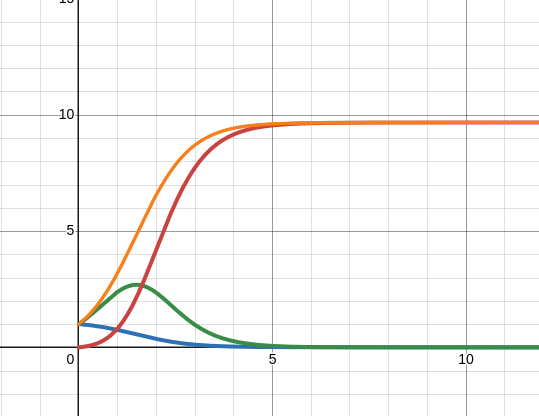
\includegraphics[width=\textwidth]{figures/IMG_ch5/QSmean/QS1} % Adjust the image path as necessary
        \caption{When $\mu = 0$.}
        \label{fig:figure1}
    \end{subfigure}
    \hspace{\fill} % Optional: adds space between figures
    % Second figure
    \begin{subfigure}{0.47\textwidth}
        \centering
        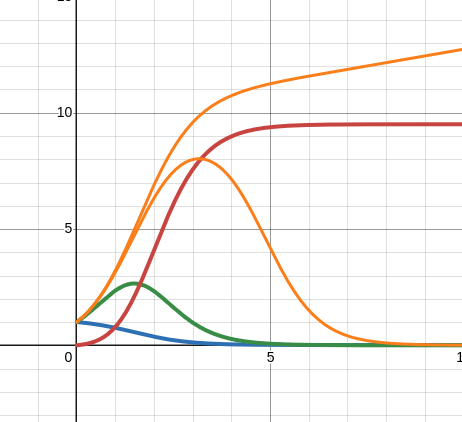
\includegraphics[width=\textwidth]{figures/IMG_ch5/QSmean/QS2} % Adjust the image path as necessary
        \caption{When $\mu > 0$.}
        \label{fig:figure2}
    \end{subfigure}
    
    \caption{In the image on the right, the conditional mean (yellow) going up at late time is the mean conditioned on $\xt \neq0$: $J(t)/\hat I(t)$. The yellow line tending to 0 is for the mean conditioned on non-catastrophe $\mean{\xt|\xt \neq R}$}
    \label{fig:two_figures}
\end{figure}



Considering the no-death $\mu = 0$ case on the left above,  it can be easily seen that the conditional mean (yellow) tends to the same limit as $V(t)$, which is shown in red.  That is 

$$\lim_{t\to\infty}     \frac{J(t)}{I(t)}     =    \lim_{t\to\infty} V(t)  = 1 + \frac{\lambda}{\delta}.$$

Here,  when $\delta$ shrinks to 0, the QS mean and expected release count tend to infinity.
